\documentclass[main.tex]{subfiles}
\begin{document}
\chapter{Analyse} 

\section{Performance}
Die Tests ergaben eine aufschlussreiche Datenmenge die wir in Hinblick auf die Performance evaluieren können. Dabei ist nicht allein der Durchsatz und Latenzzeit wichtige KPI. Es gilt ebenfalls zu analysieren ob die das Szenario von anderen ORSEs besser umgesetzt wurde. Dabei werden die Daten untereinander verglichen und mögliche Ursachen aufgezeigt. 



Aufschluss auf Java-Ausführungszeiten (Garbagecollector usw)

Memory 

Responses Compared to Other Implementation.
die Zeiten im vergleich zur 
%Overall 


% Wie ändert sich das Antwortzeitverhalten in Abhängigkeit von der Last?
% Kann mit dem System auch unter hoher Last noch akzeptabel gearbeitet werden?
% Zeigt das System undefiniertes Verhalten (z. B. Absturz)?
% Geht das System nach Rückgang der Überlast wieder in den normalen Bereich zurück?




\subsection{Durchsatz}
Wie aus der Abbildung \ref{figure:throughputSzen} ersichtlich wird sind haben alle OSRE verschiedene Durchsatzraten gezeigt. 
\newline
\textbf{Szenario 1 und 2} \newline
Der höchste Durchsatz gelang mit Apache PDFBox. Der Durchsatz war beim Szenario 1 mit der Rate von 50 virtuellen Usern auf 151 Anfragen pro Sekunde gelangt.  Apache PDFBox hat was Durchsatz und Verarbeitungsgeschwindigkeit in den ersten beiden Szenarien die höchste Rate im Vergleich zu iText und JasperReports an den Tag gelegt. 
Der Durchsatz lag bei den ersten und zweiten Szenario mit Apache PDFBox bei bei allen über 100 Anfragen pro Sekunde ausser bei den Szenarien 1b und 2b bei denen die zu verarbeitenden Daten verdreifacht wurden. 
iText zeigt ähnliche Ergebnisse dieses mal mit dem Maximum Durchsatz von 60 Anfragen pro Sekunden im Szenario 2 mit ebenfalls 50 virtuellen Usern. Der Durchsatz von iText und Apache PDFBox schwanken stark. Bei Apache PDFBox zeigte beim Vergleich vom besten Ergebnis (Szenario 1c) zum schwächsten (Szenario 1b) eine Verschlechterung des Durchsatzes von bis zu 60.9\%. Auch bei iText ist eine Vermindung des Durchsatzes festzustellen die  bis zu 83\% betrug, wenn die Ergebnisse von Szenario 2c mit denen von 1b verglichen werden. Hingegen blieb bei JasperReports mit seinem vergleichsweise schlechtem Durchsatz konstant. JasperReports zeigt bei allen Szenarien einen Durchsatz zwischen 17 und und 11 Anfragen pro Sekunden eine robustere doch langsame Implementierung des Service.\newline 
\textbf{Szenario 3}
\newline
Das dritte Szenario zeigt eine rapide Abnahme der Durchsätze. Alle drei OSRE bringen den Durchsatz nicht über 15 Anfragen pro Sekunde. Das bedeutet das im besten Fall das Szenario 3 von JasperReport 52'200 mal in einer Stunde verarbeitet werden kann. iText würde etwa 34'200 PDF in der gleichen Zeit generieren und Apache PDFBox gerade mal 18'360 PDFs liefern. 
Apache PDFBox hat in diesem Szenario die längsämste Verarbeitung mit 1.8 Anfragen pro Sekunde knap gefolgt von iText mit 3.1 Anfragen pro Sekunden. 

\begin{figure}[!ht]
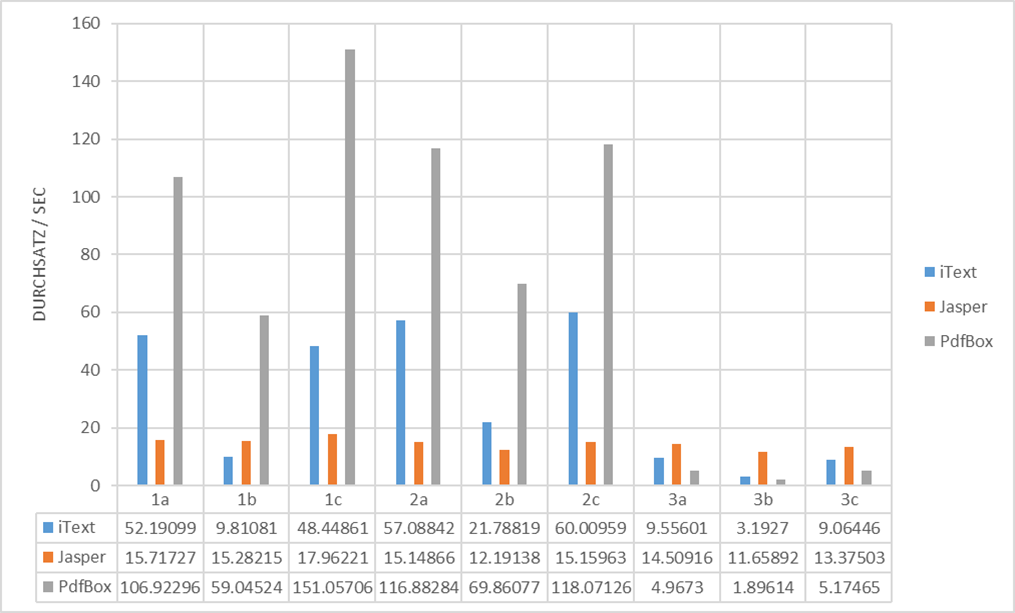
\includegraphics[width=\textwidth]{mainpart/4_analyse_img/VglDurchSzen.png}
 \caption{Vergleich - Durchsatz nach Szenario}
 \label{figure:throughputSzen}
\end{figure}


\textbf{Durchsatz nach Bytes}
Die Abbildung \ref{figure:throughputBytesAll} zeigt, dass der Durchsatz in Bytes über die Testdauer hinweg  beim Szenario 3 nicht Einbricht. 





\begin{figure}[!h]
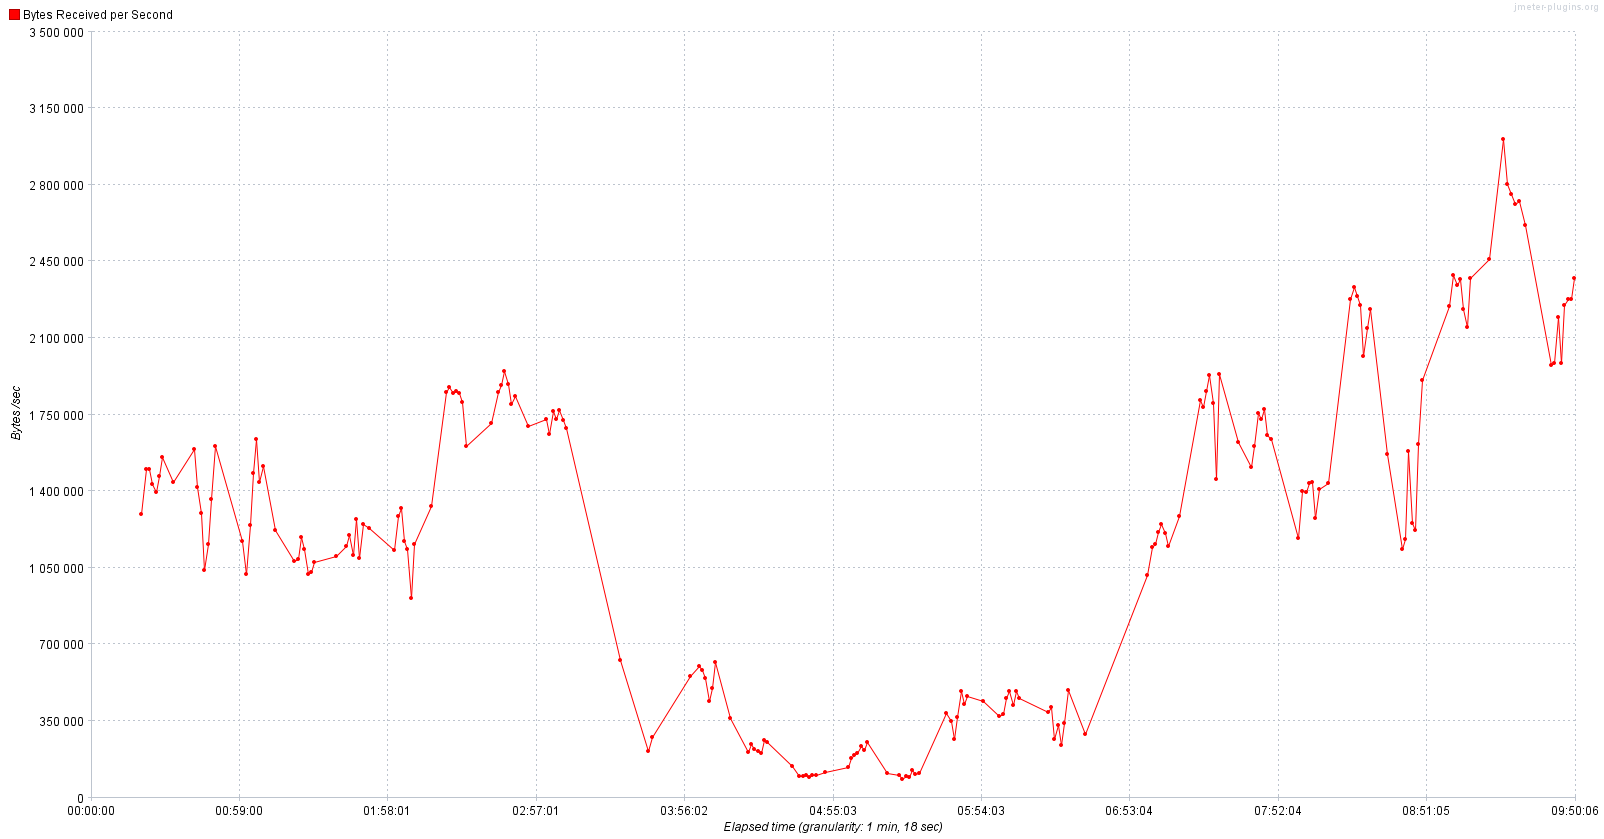
\includegraphics[width=\textwidth]{mainpart/4_analyse_img/ThroughputOverTimeAll.png}
 \caption{Durchsatz in Bytes}
 \label{figure:throughputBytesAll}
\end{figure}





\subsection{Latency}
%Min / Max Average --> Vergleichen mit anderen Projekten wer hat die kürzeste Latenz wer die längste
\begin{figure}[h]
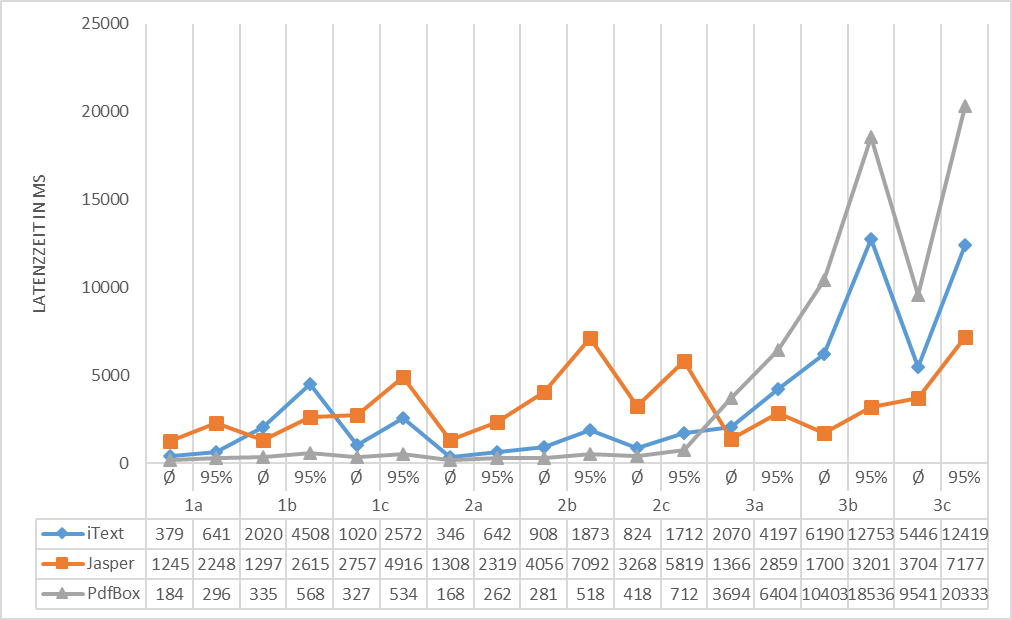
\includegraphics[width=\textwidth]{mainpart/4_analyse_img/LatenzzeitSzen.png}
 \caption{Latenzzeit nach Szenario und OSRE}
 \label{figure:latencySzenario}
\end{figure}



\begin{figure}[h]
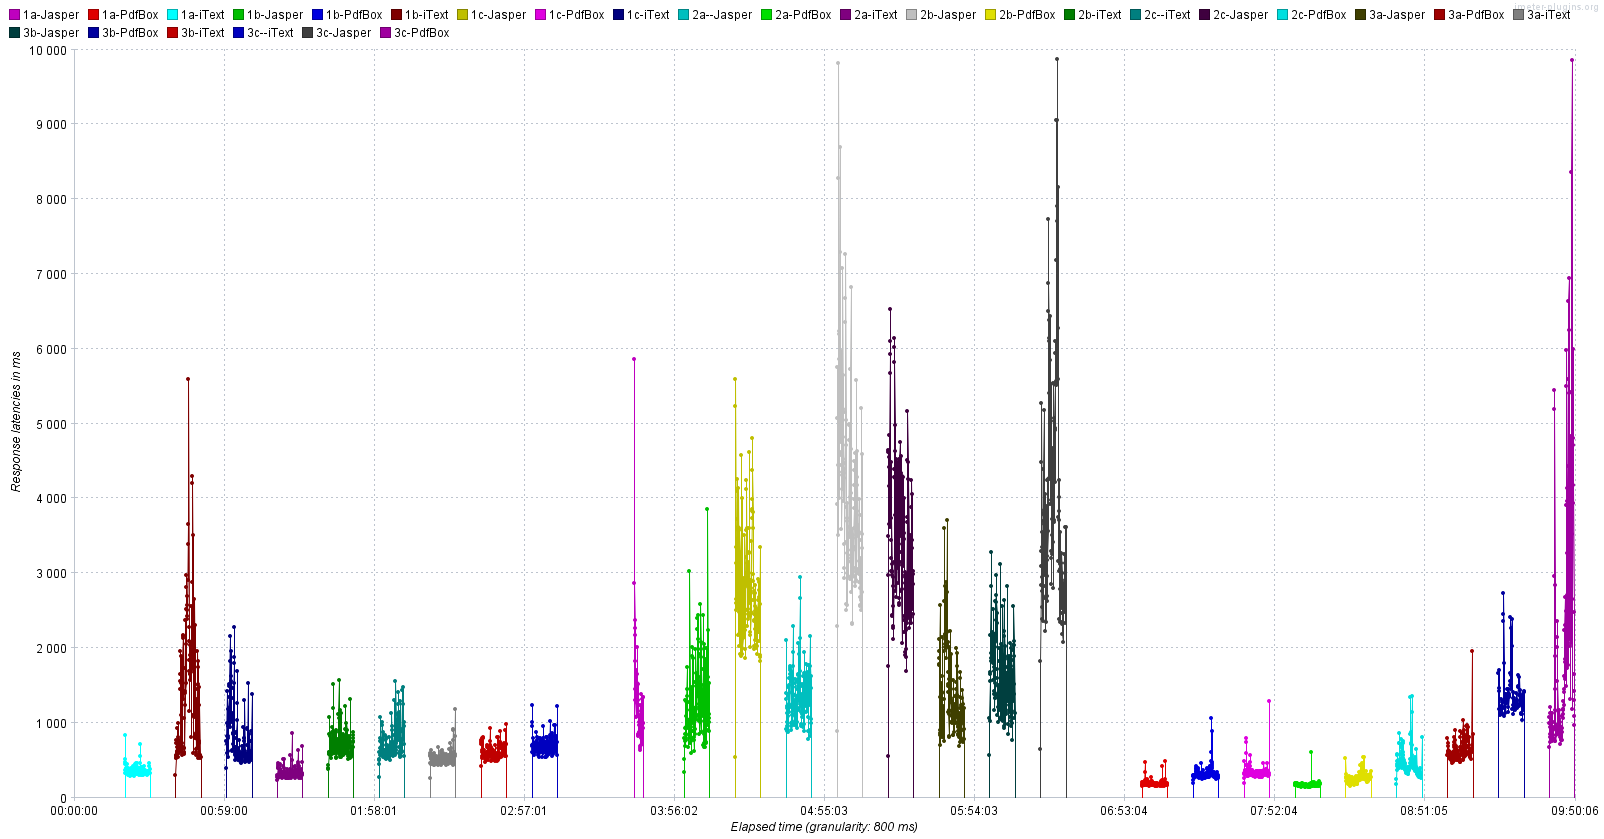
\includegraphics[width=\textwidth]{mainpart/4_analyse_img/ResponseLatenciesOverTime.png}
 \caption{Antwortzeiten Testzyklus}
 \label{figure:latencyTestcycle}
\end{figure}






\section{Monitor Resources}
\subsection{RAM}



\begin{figure}[h]
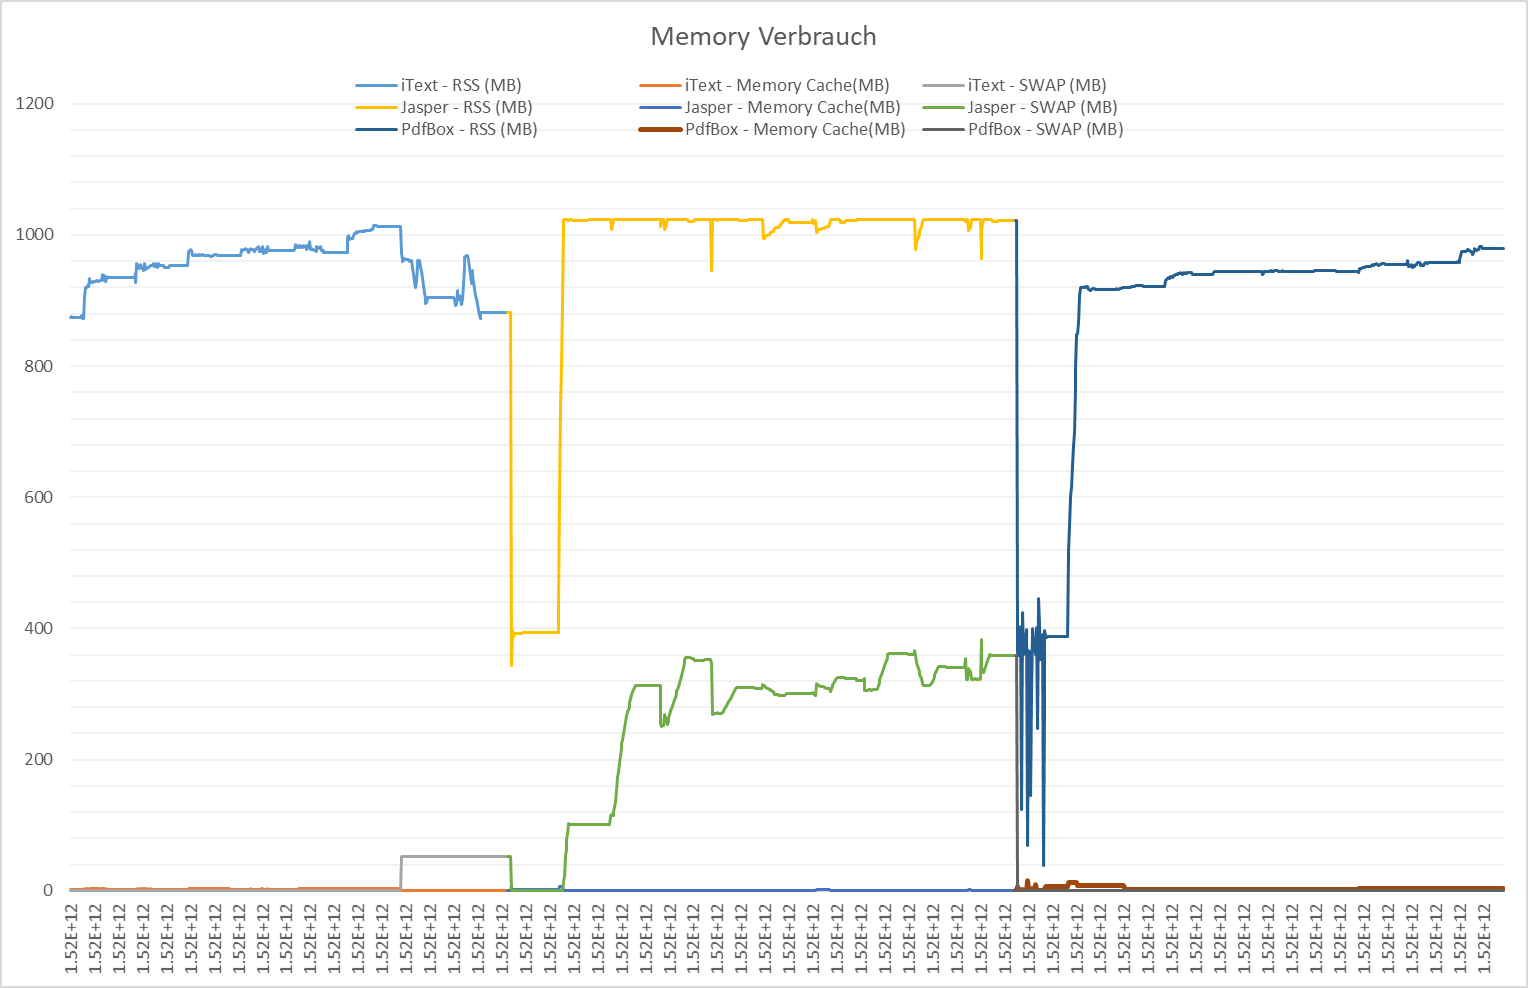
\includegraphics[width=\textwidth]{mainpart/4_analyse_img/MemoryVerbrauch.png}
 \caption{Memoryverbrauch Testlauf}
 \label{figure:memorytestlauf}
\end{figure}




\section{Reporting Engines - Vergleich}


Die OSRE haben sich wärend den Test, in Bezug auf Latenzzeit und Ressourcenverbrauch, verschieden verhalten. In diesem Kaptel sollen die  

\subsection{Requestgrösse}

Im Vergleich zu den Szenarien 1a, 2a und 3a wurden bei den Szenarien 1b, 2b und 3b die Datensätze für die Verarbeitung verdreifacht. Wie aus den Auswertungen und Abbildungen (siehe Abbildung \ref{figure:vglReqitext}, \ref{figure:vglReqjasper} und \ref{figure:vglReqPdfBox}) entnommen werden kann hat die dazu geführt das sich alle Antwortzeiten und Durchsätze verschlechtert haben.

Die OSRE und iText und Apache PDFBox haben sich in der gleichen Art und Weise verschlechtert. Diese haben bei den Szenarien 1 und 2 einen Rückgan

Hier sei noch einmal hervorgehoben dass diese Daten aufgrund eines Testlaufs ermittelt wurden, es kann in jedem Testlauf das gleiche Phänomen beobachtet werden, dennoch sind diese Daten nicht stellvertretend oder absolut zu betrachten, grösserer Ausreisser wurden in anderen Testläufe aufgezeichnet was die Tatsache unterstreicht dass die Infrastruktur nicht schwankungsfrei.


\begin{figure}[!ht]
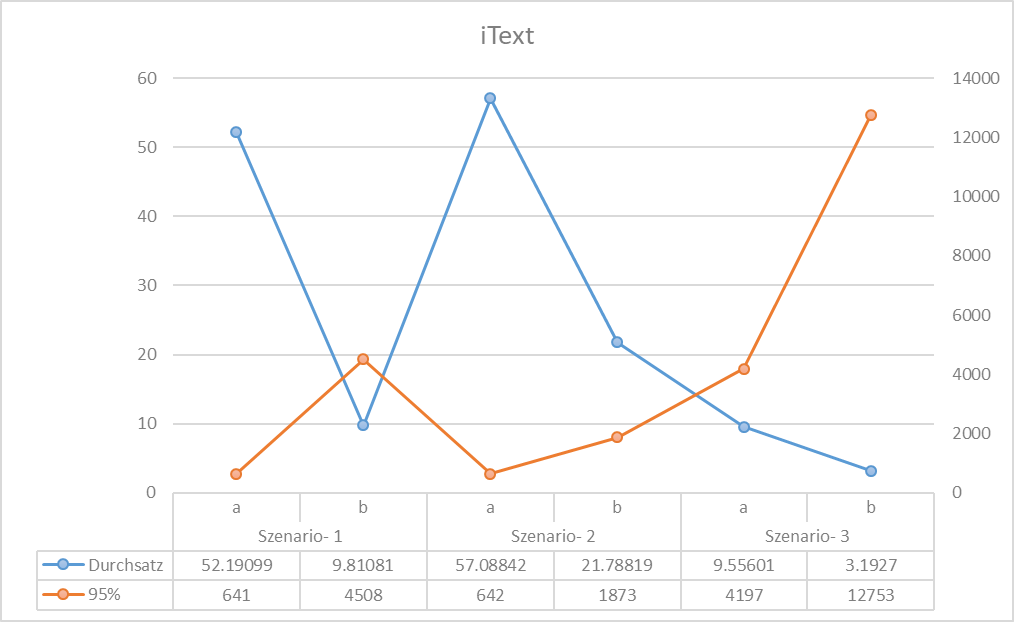
\includegraphics[width=\textwidth/2]{mainpart/4_analyse_img/iText_ab.png}
 \caption{iText - Vergleich  Request-Grösse Performance}
 \label{figure:vglReqitext}
\end{figure}

\begin{figure}[ht]
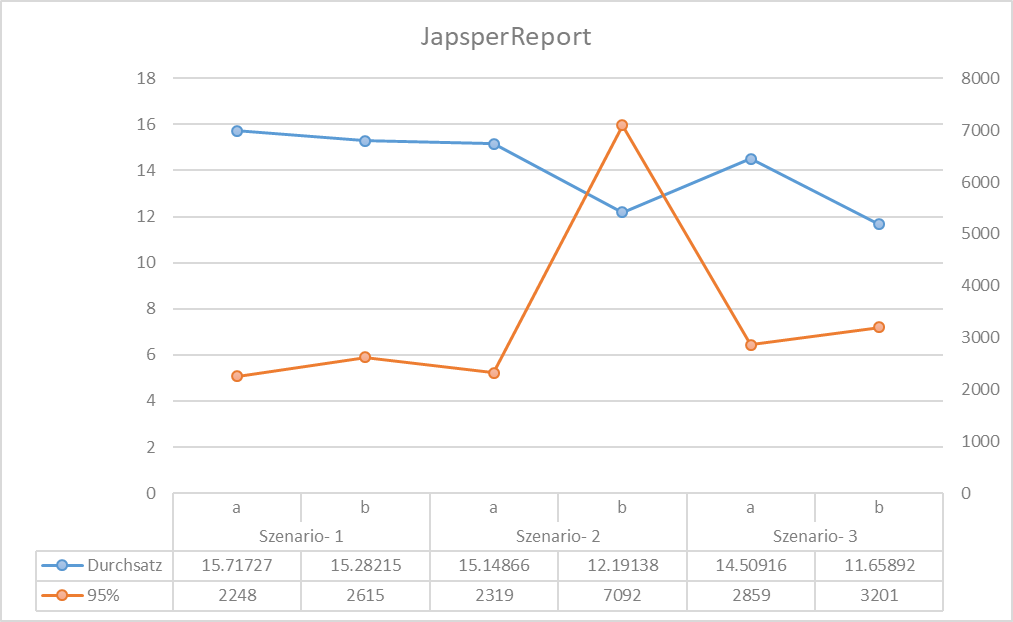
\includegraphics[width=\textwidth/2]{mainpart/4_analyse_img/Jasper_ab.png}
 \caption{JasperReports - Vergleich Request-Grösse Performance }
 \label{figure:vglReqjasper}
\end{figure}

\begin{figure}[ht]
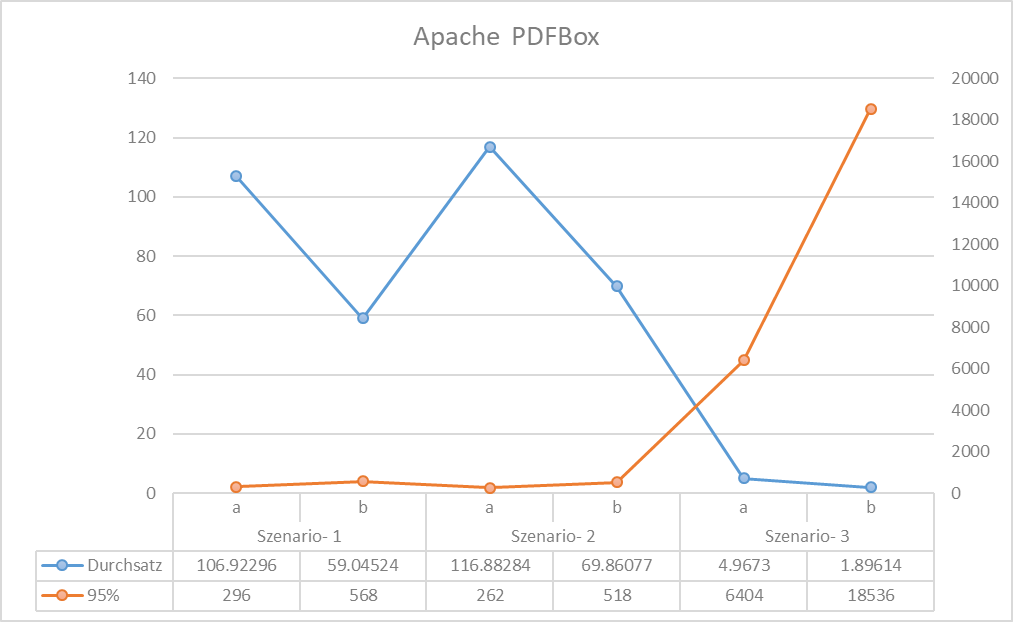
\includegraphics[width=\textwidth/2]{mainpart/4_analyse_img/PdfBox_ab.png}
  \caption{Apache PDFBox - Vergleich Request-Grösse Performance}
 \label{figure:vglReqPdfBox}
\end{figure}




\subsection{Virtuelle User}

\begin{figure}[h]
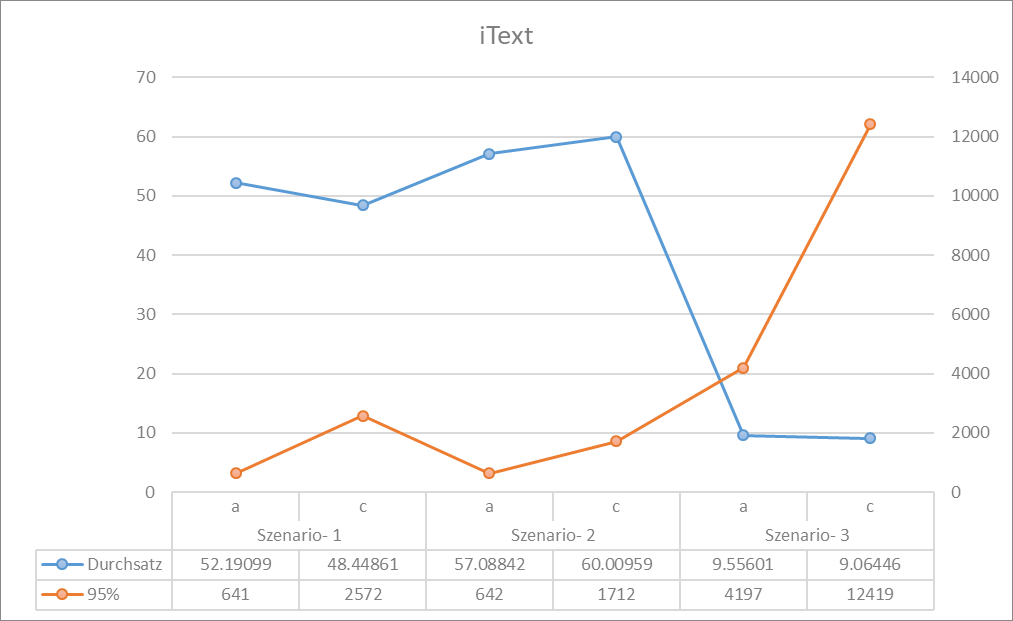
\includegraphics[width=\textwidth/2]{mainpart/4_analyse_img/iText_ac.png}
 \caption{iText - Vergleich virtuelle User Performance}
 \label{figure:vglVUitext}
\end{figure}

\begin{figure}[h]
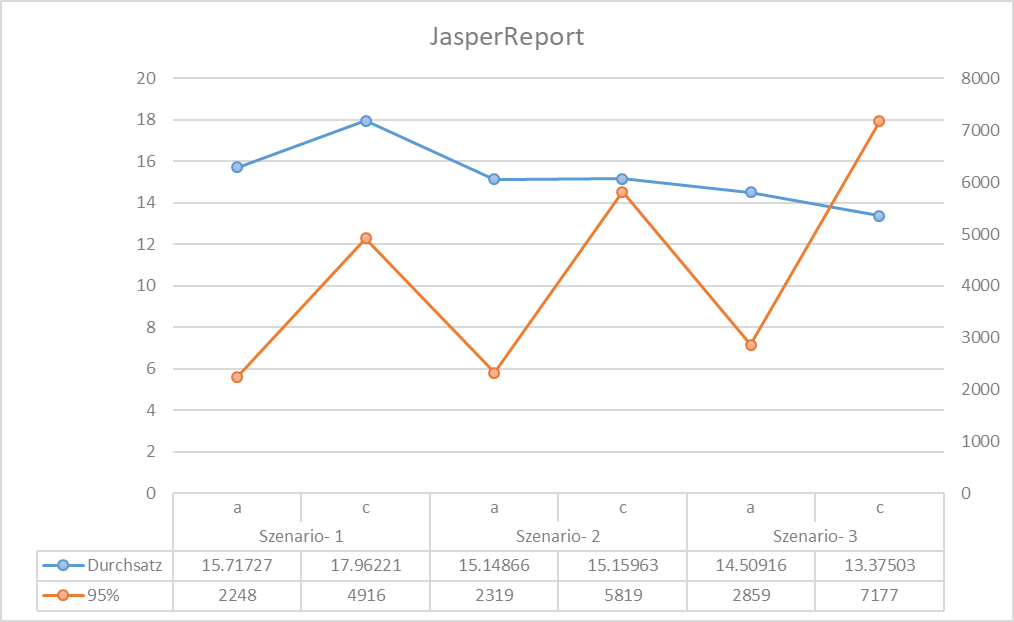
\includegraphics[width=\textwidth/2]{mainpart/4_analyse_img/Jasper_ac.png}
 \caption{JasperReports - Vergleich virtuelle User Performance }
 \label{figure:vglVUjasper}
\end{figure}

\begin{figure}[h]
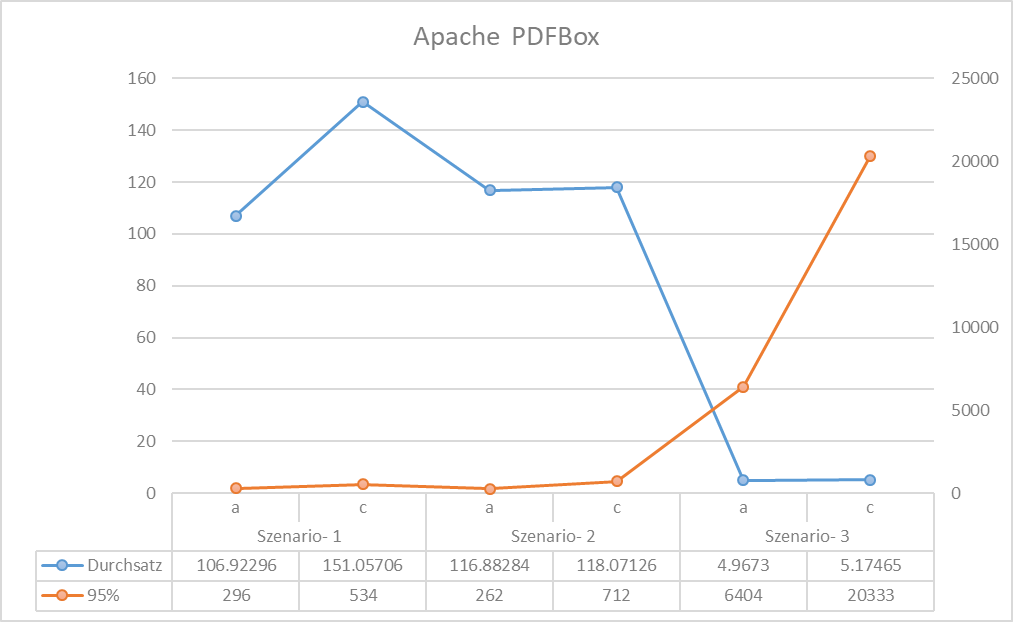
\includegraphics[width=\textwidth/2]{mainpart/4_analyse_img/PdfBox_ac.png}
  \caption{Apache PDFBox - Vergleich virtuelle User Performance}
 \label{figure:vglVUPdfBox}
\end{figure}



\textbf{Memory}
\textbf{Throughput}
\textbf{Latenz}

\subsection{Mehr Virtuelle User}
\begin{figure}[h]
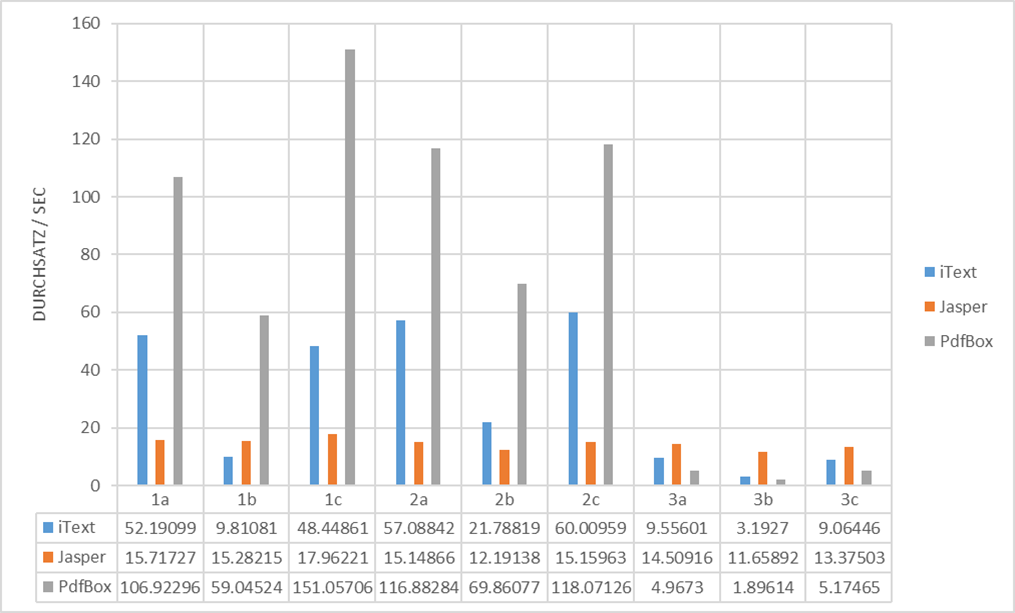
\includegraphics[width=\textwidth]{mainpart/4_analyse_img/VglDurchSzen.png}
 \caption{Vergleich - Durchsatz nach Szenario}
 \label{figure:througputSzenario}
\end{figure}


\textbf{Memory}
\textbf{CPU}
\begin{figure}[h]
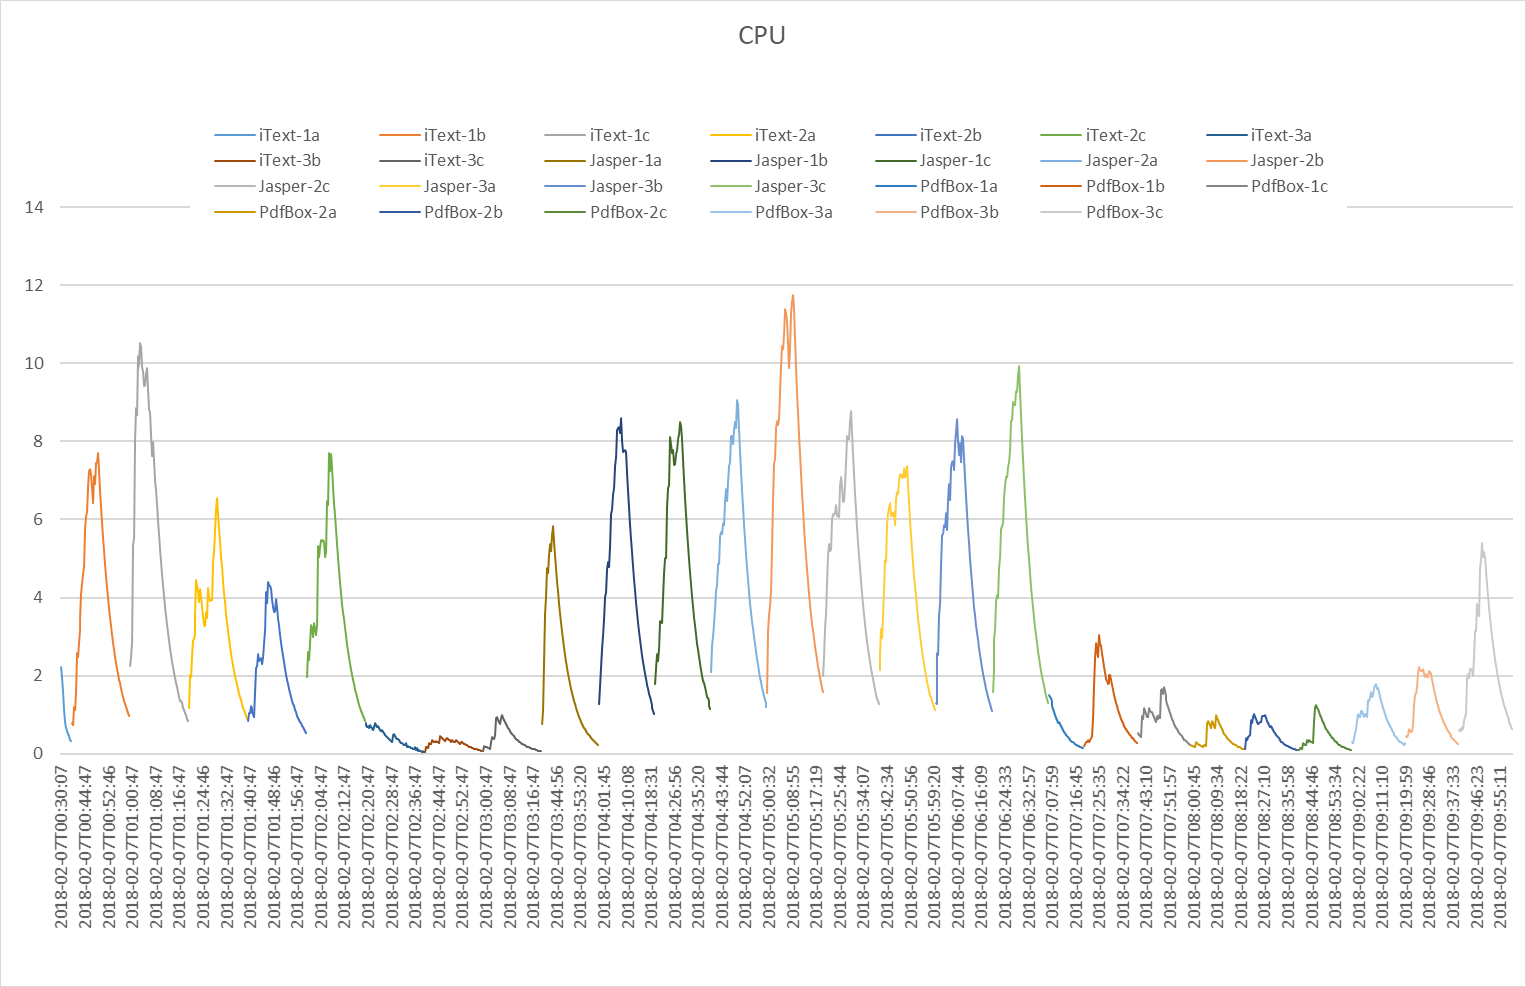
\includegraphics[width=\textwidth]{mainpart/4_analyse_img/CPUVergleich.png}
 \caption{Vergleich - Durchsatz nach Szenario}
 \label{figure:cpuVergleich}
\end{figure}

\subsection{Vergleich der Szenarien innerhalb eines Projektes}

\textbf{Apache Pdf Box}

% Grafik 
% Text was sehen wir
\textbf{iText}
% Grafik 
% Text was sehen wir
\textbf{Jasper Report}
% Grafik 
% Text was sehen wir
\subsection{Verglich der Szenarien mit den anderen Projekten }


\subsubsection{Szenario 1}

% Grafik 

% Was sehen wir 

% Warum sehen wir das?

\subsubsection{Szenario 2}
% Grafik 

% Was sehen wir 

% Warum sehen wir das?
\subsubsection{Szenario 3}
% Grafik 

% Was sehen wir 

% Warum sehen wir das?



\section{Ursachenanalyse}

Im Szenario 3 konnte man den Rückgang von iText und Apache PDFBox erkennen. Es lässt sich anhand der Ergebnisse der verschiedenen Metriken die  Schlussfolgerung gezogen werden, dass der Durchsatz nicht durch eine Netzwerk- oder Infrastrukturstörung herbeigeführt wurde. Es ist fraglich ob das sich diese schlechte Performance einen Zusammehang mit anderen nicht beinflussbaren Einflussfaktoren haben können. Dennoch zeigt sich einerseits das die Implementierung im Zusammenhang mit dem Szenario 3 zur Generierung von Vergleichsweise grossen PDFs führte. andererseits ist der Aufbau und Layout bei iText und Apache PDFBox mit mehr Rechenleistung verbunden. Apache PDFBox zeigt bei der Last auf dem PaaS-Provider höhere Last bei der Ausführung des Szenario 3. iText wiederum zeigt keine Zuname sondern sogar einen Rückgang der CPU-Last. 



















\end{document}